\documentclass{article}
\usepackage[utf8]{inputenc}
\usepackage{hyperref}
\usepackage{graphicx}

\hypersetup{
    colorlinks=true,
    linkcolor=blue,
    filecolor=magenta,      
    urlcolor=cyan,
    pdftitle={Overleaf Example},
    pdfpagemode=FullScreen,
    }




\title{Research Paper Summary - IoT Architecture, Application Protocols and Energy Needs}
\author{Adithi Iyer}
\date{January 2023}

\begin{document}

\maketitle

\section{IoT Architectures and Protocols - Research Paper Summary}

\subsection{IoT 4 layer Architecture}

\begin{figure}[h!]
    \centering
    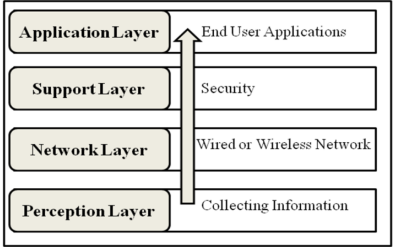
\includegraphics[width=\linewidth]{4LayerArch.PNG}
    \caption{IoT - 4 Layer Architecture}
    \label{fig:my_label}
\end{figure}

An IoT architecture typically consists of four layers: the perception layer, the network layer, the support layer, and the application layer.

The perception layer is made up of the physical devices and sensors that collect data. These devices are often low-power and have limited processing capabilities.


The network layer is responsible for connecting the devices to the internet and enabling communication between them. This layer includes the various networking protocols used for IoT, such as Zigbee, Z-Wave, and Bluetooth Low Energy (BLE).


The support layer is introduced in the 4 layer architecture for security purposes. The reason to make a fourth layer is the security in architecture of IoT. Information is sent directly to the network layer in three-layer architecture. Due to sending information directly to the network layer, the chances of getting threats increase.


The application layer is the topmost layer, where the data is used to create value for the end user. This layer includes the various applications and services that are built on top of the support layer to provide specific functionality, such as remote monitoring and control, data visualization, and analytics.








\subsection{IoT 5 layer Architecture}

\begin{figure}[h!]
    \centering
    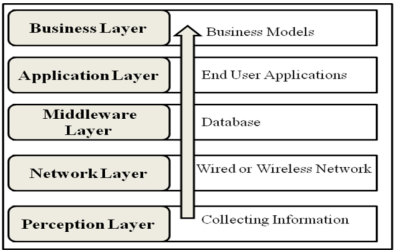
\includegraphics[width=\linewidth]{5LayerArch.PNG}
    \caption{IoT - 5 Layer Architecture}
    \label{fig:my_label}
\end{figure}

In case of the architecture of IoT in five layers: the perception layer, the network layer, the middleware layer, the application layer and the business layer.

The Perception layer, Network layer and Application layer is similar to that seen in the 4 layer architecture of IoT.


The Perception Layer is the lowest layer and includes the physical devices and sensors that collect data. It deals with sensing and data acquisition from the physical environment.


The Network Layer connects the devices to the internet and includes protocols such as IPv4 and IPv6, as well as various routing protocols. It is responsible for communication between devices, gateways and the cloud.


The Middleware Layer provides the infrastructure for storing, processing and analyzing the data collected by the devices. It includes cloud platforms such as AWS, Azure, and Google Cloud, as well as edge computing platforms. It acts as a bridge between the perception and application layers, and it provides a common interface to access the raw data.


The Application Layer is the top layer and includes the applications and services that are built on top of the platform and network layers to provide specific functionality for the end-user. It includes the algorithms, data analytics, and decision-making processes that are executed on the data received from the perception layer


The Business Layer includes the applications and services that are built on top of the platform and network layers to provide specific functionality for the end-user. It includes the business logic and processes that are executed on the data received from the application layer. It is used to create value and revenue from the IoT systems.



\subsection{IoT Protocols}

\begin{figure}[h!]
    \centering
    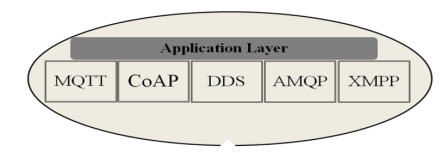
\includegraphics[width=\linewidth]{appLayerProtocols.PNG}
    \caption{IoT - Application Layer Protocols}
    \label{fig:my_label}
\end{figure}

Each layer has its own set of protocols and technologies to enable communication and data flow.

TCP/IP (Transmission Control Protocol/Internet Protocol) is a set of communication protocols that are used to connect devices on the internet.TCP/IP is used to connect IoT devices to the internet and to each other. TCP is a transport-layer protocol that is responsible for establishing connections between devices, breaking data into packets, and ensuring that the packets are delivered reliably and in the correct order. IP is a network-layer protocol that is responsible for routing packets of data between devices. It uses IP addresses to identify devices on the network and to determine the best path for data to travel. Together, TCP and IP enable devices to communicate with each other and share data across the internet.

MQTT (Message Queuing Telemetry Transport) is a publish/subscribe based messaging protocol for use on top of the TCP/IP protocol. MQTT is a lightweight messaging protocol that provides resource-constrained network clients with a simple way to distribute telemetry information.

CoAP (Constrained Application Protocol) is a software protocol intended to be used in very simple electronics devices that allows them to communicate interactively over the Internet. CoAP is designed to easily translate to HTTP for simplified integration with the web.

XMPP (Extensible Messaging and Presence Protocol) is a communications protocol for message-oriented middleware based on XML (Extensible Markup Language).

DDS (Data Distribution Service) is a publish/subscribe protocol that is designed for real-time data distribution in distributed systems. It enables devices to send and receive data in a reliable and efficient manner, and it includes features such as discovery, quality of service, and security. DDS is often used in IoT systems to enable real-time communication and data sharing between devices.

AMQP (Advanced Message Queuing Protocol) is a messaging protocol that is designed to provide a reliable and flexible messaging infrastructure for distributed systems. It enables devices to send and receive messages asynchronously, and it includes features such as routing, reliability, and security. AMQP is often used in IoT systems to enable asynchronous communication and data sharing between devices.

XMPP (Extensible Messaging and Presence Protocol) is an open standard communication protocol for message-oriented middleware based on XML (Extensible Markup Language). It is designed for real-time, extensible and decentralized communication. It enables devices to send and receive messages and presence information in a reliable and efficient manner, and it includes features such as instant messaging and presence. XMPP is often used in IoT systems to enable real-time communication and data sharing between devices.

All of these protocols are designed to provide reliable communication and data sharing between devices and they can be used depending on the specific requirements of the IoT system. 

\subsection{Energy}
 The article discusses the issue of energy efficiency in IoT and the different algorithms and approaches that researchers are using to overcome this issue. These approaches include the use of the AODV protocol(Ad-hoc On-demand Distance Vector: a loop-free routing protocol for ad-hoc networks) for shortest path data transmission and the Adaptive Duty Cycle (ADC) Algorithm for energy consumption. The paragraph also mentions the use of RFID, WSN, and RSN for data transmission in IoT networks and the effect of energy efficiency on network performance. The authors mention about the Green-IoT concept, which is a new vision for power-down mechanisms and energy-efficient communication in IoT networks. They also mention about the different conflicts that researchers face like AODV protocol's delay time, which is increased slightly and the probability is decreased. In addition, they propose the use of LPWAN(Low-Power Wide-Area Network) and adaptive techniques such as ADC and channel allocation using adaptive reinforcement learning algorithms for a green IoT environment. Finally, the text also discusses the area of IoT device security with energy using encryption methodology and a new method called SeLPC(Secure Low Power Communication) that can reduce power consumption by 26.2%.

\section{Reference Research Paper}


\href{https://drive.google.com/file/d/1bUMbR2HERnViNIY0Zxo2yNvXsN4xiVm9/view?usp=sharing}{\textbf{Study on IoT Architecture, Application Protocol and Energy needs}}

\textbf{Poorana Senthilkumar S}

\textit{Dr. N.G.P. Arts and Science College}

\textbf{Bhavadharani Subramani}

\textit{K S RANGASAMY COLLEGE OF ARTS AND SCIENCE (AUTONOMOUS)}


\end{document}
